\documentclass{article}

\usepackage{icmc2017template}
\usepackage{amsmath}
\usepackage{amssymb}
\usepackage{soul}
\usepackage{microtype}
\usepackage{csquotes}
\usepackage{polyglossia}
\usepackage{footmisc}
\setmainfont{Times New Roman}

\setdefaultlanguage{english}
\usepackage{tikz}
\usepackage{listings}
\usepackage{subcaption}
\usepackage{booktabs}
\usepackage{enumitem}\setlist{nosep}
\setitemize{itemsep=1pt}

\usepackage[backend=biber]{biblatex}
\addbibresource{biblio.bib}

\def\papertitle{Extending dataflows with temporal graphs}
\def\firstauthor{Jean-Michaël Celerier}
\def\secondauthor{Myriam Desainte-Catherine}
\def\thirdauthor{Jean-Michel Couturier}

\threeauthors
{0.5in}
{\firstauthor} {LaBRI, Blue Yeti \\
    Univ. Bordeaux, LaBRI, UMR 5800, ~\\ F-33400 Talence, France. \\  Blue Yeti, F-17110 France. \\ jcelerie@labri.fr}
{\secondauthor} {LaBRI, CNRS \\ Univ. Bordeaux, LaBRI, UMR 5800, ~\\ F-33400 Talence, France. \\ CNRS, LaBRI, UMR 5800, ~\\F-33400 Talence, France. \\  INRIA, F-33400 Talence, France. \\ myriam@labri.fr}
{\thirdauthor} {Blue Yeti, F-17110 France. \\ jmc@blueyeti.fr}

\DeclareMathOperator{\commit}{commit}
\DeclareMathOperator{\pull}{pull}
\usepackage[explicit]{titlesec}
\lstset{basicstyle=\ttfamily\footnotesize,breaklines=true}


\titleformat{name = \section, numberless}[runin]
{\bfseries}
{}
{1em}
{#1}

\usepackage[
pdftitle={\papertitle},
pdfauthor={\firstauthor, \secondauthor, \thirdauthor},
bookmarksnumbered, % use section numbers with bookmarks
pdfstartview=XYZ % start with zoom=100% instead of full screen; 
% especially useful if working with a big screen :-)
]{hyperref}
%\pdfcompresslevel=9

\usepackage{graphicx}
\DeclareGraphicsExtensions{.pdf,.jpeg,.png}

\usepackage[figure,table]{hypcap}


\hypersetup{
    colorlinks,%
    citecolor=black,%
    filecolor=black,%
    linkcolor=black,%
    urlcolor=black
}

\title{\papertitle}

%%%%% TODO pour review
%% Ok: Parler de Bach et du truc du mec de l'IRCAM (dynamic patching en lisp)
%% Ok: Expliquer que ce n'est pas qu'un mécanisme pour patcher Pd; à venir: objets de i-score.
%% Présenter ça comme la fusion du modèle flot de données et du modèle séquenceur comme dans Ableton + Max For Live
%% Différence avec patching dynamique: l'agencement temporel des objets entre eux peut être statique.
%% Expliquer les raisons: 
%% Mettre accent sur aspects temporels
%% Ok:  Expliquer qu'on présente un paradigme, qu'il est implémenté à bas niveau dans la libossia et à haut niveau dans i-score (dont l'intégration avec Pd)
%% Bof: Accentuer le fait qu'il n'y ait pas besoin de coder
%% Bof: Définir la notion de dynamicité utilisée.
%% Bof: "Any other system of temporal relationships" : donner examples. Par ex. Antescofo, etc ?
%% Ok: Expliquer implémentation: mettre capture d'écran ?

%% User evaluation... bof
\begin{document}
    
\capstartfalse
\maketitle
\capstarttrue
\begin{abstract}
    Numeric musical and artistic creation is in great part based on well-known patcher softwares: Max/MSP, PureData, OpenMusic, vvvv\dots 
    
    Yet, handling temporal evolutions and structures on large scales remains a central problem: for instance, writing a song with introduction, chorus, verse, chorus, parts in Max presents many hurdles to the composer.    
    Hence, multiple software have introduced tracks and automations to provide a temporal control of a given set of parameters in a single or even multiple concurrent time-lines.
    
    We present an extension to the dataflow paradigm used by patchers that allows to handle the execution of any parts of a computation in time. 
    That is, instead of sending control messages to existing patchs, they are run in a time-line which orchestrates the data bindings between different parts of the dataflow. 
    This enables dynamic behaviours when creating temporal compositions. An example is given with Pure Data patches and an i-score scenario.
\end{abstract}
    
\section{Introduction}
This work explores the association of macroscopic temporal semantics with the dataflow graphs generally used in music and signal processing.
    
We analyze the meanings that can be given to processes executing in time, when these processes have a data dependency and do not execute at exactly the same time.
    
For instance, given two processes $p_1, p_2$, what can be said of a program where $p_1$ executes from $t=0$ to $t=5$ seconds, and $p_2$ from $t=3$ to $t=6$ when $p_1$ and $p_2$ operate on the same data?
    
An example would be an audio filter: $p_1$ is a low-pass and $p_2$ a reverb; we want the reverb to activate only after an action of a performer and stop after a few seconds.
    
The simplest strategy can be to only allow execution when all processes are active and have been given a definite order of execution: in this case the overall program will only execute during the intersection of the activation of $p_1$ and $p_2$, which goes from $t=3$ to $t=5$. 
While safe from the point of view of software execution, we will show that other execution policies leveraging information from the temporal layout of the processes can provide composers with new creative capabilities, through an example that uses Pure Data.
    
An environment associated with the dataflow graph is introduced; it contains the values of the inputs and outputs of the processes in this graph.
Then, since a graph may not always be fully active, we show that it is also meaningful to have implicit connections between nodes of the graph, that will use the environment.
This allows dynamic routing of the processes according to their temporal order during execution, and extends routing to pattern-matched elements of the environment instead of single values.
Three different behaviors between the input and output parameters of the dataflow nodes are presented: strict, glutton, and delayed. 

\begin{figure} [h]
	\centering
	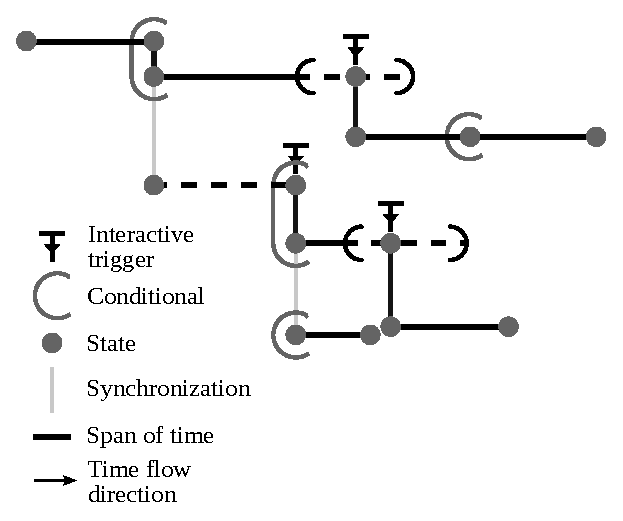
\includegraphics[width=0.35\textwidth]{images/iscore-example.eps}
	\caption{Part of an OSSIA scenario, showcasing the temporal syntax used. 
		A full horizontal line means that the time must not be interrupted, 
		while a dashed horizontal line means that the time of this time constraint can be interrupted to proceed 
		to the following parts of the score according to an external event.}
	\label{fig.iscore-example}
\end{figure}

\subsection{Related works}
There is a long-standing interest in the handling of time in programming languages, which is intrinsically linked to how the language handles dynamicity.

PEARL90\cite{halang2001safe}\footnote{Not to be mistaken with the Perl language commonly used for text processing} provides temporal primitives allowing for instance to perform loops at a given rate for a given amount of time.
More recently, Céu has been introduced as a synchronous language with temporal operators, and applications to multimedia\cite{Santos:2016:CLI:2976796.2976856}.

OpenMusic is a visual environment which allows to write music by functional composition.
It has been recently extended with timed sequences allowing to specify evolutions of parameters in time\cite{garcia:hal-01484077}.

Likewise, the Bach library for Max~\cite{agostini2015max} allows to define temporal variations of parameters during the playing of a note by with the mechanism of slots.
The processes controlled by such parameters are then available to use in the Max patch.

The Max for Live extension to Ableton Live allows to embed Max patches in the Ableton Live sequencer. 
Through the API provided, one can control the execution of various elements of the sequencer in Max; automations in Live can also be used to send data to Max patches at a given time.

A method for dynamic patching of Max abstractions based on CommmonLisp has been proposed by Thomas Hummel\cite{hummel1994common} to reduce resource usage by enabling and disabling sub-patches at different points in the execution of a program.
This has the advantage of saving computing power for the active elements of the score.

Dataflows and especially synchronous dataflows have seen tremendous usage in the music and signal processing community. 
A list of patterns commonly used when developing dataflow-based music software is presented in~\cite{arumi2006dataflow}.
Formal semantics are given in~\cite{benveniste_data-flow_1993}.
Specific implementation aspects of dataflow systems are discussed in the Handbook of Signal Processing Systems\cite{bhattacharyya_handbook_2013}. 

Dynamicity in dataflows is generally separated in two independent aspects: dynamicity of the data, and of the topology.
The first relates to the variability on the streams of tokens, while the second is about changes to the structure of the graph. 
Boolean parametric dataflows\cite{bempelis2015boolean} have been proposed to solve dynamicity of topology, by introducing conditionals at the edges.

\subsection{Temporal formalism}

This work implicitly uses the OSSIA formalism~\cite{celerier2015ossia} in its examples to provide primitives relative to the evolution of time: time constraints (horizontal lines), time nodes (vertical lines). 
The elements of its syntax are presented in fig.~\ref{fig.iscore-example}.

It is important to note that any other system of temporal relationships between processes could be used instead.

\section{Definitions}
\begin{figure}[h]
	\centering
	\begin{subfigure}{0.15\textwidth}\centering
		\begin{tikzpicture}[scale=0.5]
		\node[draw, circle] (f1) at (0, 0) { $f_1$ };
		\node[draw, circle] (f2) at (3, 0) { $f_2$ }
		edge [<-] (f1);
		\end{tikzpicture}\caption{}\label{fig.f1tof2}
	\end{subfigure}~
	\begin{subfigure}{0.15\textwidth}\centering	
		\begin{tikzpicture}[scale=0.5]
		\node[draw, circle] (f1) at (0, 0) { $f_1$ };
		\node[draw, circle] (f2) at (3, 0) { $f_2$ }
		edge [->] (f1);
		\end{tikzpicture}\caption{}
	\end{subfigure}~	
	\begin{subfigure}{0.15\textwidth}\centering
		\begin{tikzpicture}[scale=0.5]
		\node[draw, circle] (f1) at (0, 0) { $f_1$ };
		\node[draw, circle] (f2) at (3, 0) { $f_2$ };
		\end{tikzpicture}\caption{}
	\end{subfigure}
	\caption{Possible dataflows between $f_1$ and $f_2$. 
		As can be seen in fig.~\ref{fig.tgraph}, there are no relationships between $f_1$ and $f_2$ in the temporal graph.}
	\label{fig.simple-dataflow}
\end{figure}

We call process an entity that consists in a function $f$, an associated state, any number of inputs and output ports, and an activation status.
$f$ has a single argument $t \in \mathbb{R^+}$.
The execution of $f$ may read any number of tokens from the inputs and write any number of tokens to the outputs.
    
The function associated to an inactive process may not be executed.

We rely on two families of graphs for defining the execution of a program:
    
\begin{itemize}
  \item Synchronous dataflow graphs between processes:~\\$G_d(V_d, E_d)$ where $V_d$ is the set of processes and $E_d$ the set of data bindings between processes.
	
  \item Temporal graphs, based on the OSSIA formalism: $G_t(V_t, E_t)$ where $V_t$ is the set of time nodes and $E_t$ is the set of time constraints in a score. 
  For coherency, we call these graphs temporal graphs.
\end{itemize}

In the following, we consider a program consisting in a dataflow, and a temporal graph.
    
A program may consist in more than a single temporal graph: they are defined as processes themselves, which provides them with time information.
    
Each time constraint has an associated set of references to processes.
A process may only be executed if it is referenced at least once in a time constraint, 
at the exception of a special ``main'' process that acts as an entrypoint.
    
The execution of a program is synchronous and driven by a scheduler.
At each tick, the state of each temporal graph is updated with the following informations:
    
\begin{itemize}
  \item Which processes are currently activated.
  \item For how long these processes have been activated.
\end{itemize}

This is done according to the various events that occur and may change the order of activation of processes.

Processes are then sorted according to their dependencies and activation status, and finally executed.
% In a given tick, every active process will be executed. ?
%Event-driven vs time-driven vs sound-driven ; each node has a "driver" port which is the time or the sound. (Do like LV2: pass empty buffers). Pb: multi-rate ... voir méthode pour passer de multi-rate à single rate dans PLOP2006 et Signal Flow Graphs and Data Flow Graphs (3.2, 3.3), dans Handbook of Signal Processing (First Edition)
    
% Pour thèse: essayer de spécifier l'ensemble des cas possible / configuraitons d'activation de manière statique à partir d'un scénario donné, même si c'est exponentiel..

%\subsection{Why multiple graphs ?}
%\subsection{Hierarchy}
    
Throughout this paper, we will use the execution traces in fig.~\ref{fig.simple} and fig.~\ref{fig.simple-reversed} as running example, as well as the relationships between $f_1$ and $f_2$ present in fig.~\ref{fig.simple-dataflow}. 
    
\begin{figure}[h]

\centering
\begin{tikzpicture}[]
\definecolor{mygrey}{RGB}{100,100,100}
\draw[line width=1pt] (0, 17.1595)  -- (0, 15.6265) ; % TimeNode.0 
\draw[line width=1pt] (1.64502, 17.1595)  -- (1.64502, 17.1595) ; % drag29wine94 
\draw[line width=1pt] (5, 17.1595)  -- (5, 17.1595) ; % slid38maya79 
\draw[line width=1pt] (1.47186, 15.6265)  -- (1.47186, 15.6265) ; % glut76duff98 
\draw[line width=1pt] (4.85554, 15.6265)  -- (4.85554, 15.6265) ; % ouch30vade32 
\draw[dashed,line width=1pt] (0, 17.1595)  -- (1.64502, 17.1595) ; % gaur3skin98 
\draw[line width=1pt] (1.64502, 17.1595)  -- (5, 17.1595) ; % f1 
\draw[line width=1pt] (1.64502, 17.0595) rectangle (5, 16.0595) node[pos=.5] {$f_1$};
\draw[dashed,line width=1pt] (0, 15.6265)  -- (1.47186, 15.6265) ; % mail74chic13 
\draw[line width=1pt] (1.47186, 15.6265)  -- (4.85554, 15.6265) ; % f2 
\draw[line width=1pt] (1.47186, 15.5265) rectangle (4.85554, 14.5265) node[pos=.5] {$f_2$};

\fill[color=mygrey] (0, 17.1595) circle (0.075) ; % State.0 
\fill[color=mygrey] (1.64502, 17.1595) circle (0.075) ; % State.1 
\fill[color=mygrey] (5, 17.1595) circle (0.075) ; % State.2 
\fill[color=mygrey] (0, 15.6265) circle (0.075) ; % State.3 
\fill[color=mygrey] (1.47186, 15.6265) circle (0.075) ; % State.4 
\fill[color=mygrey] (4.85554, 15.6265) circle (0.075) ; % State.5 
\end{tikzpicture}
\caption{The example temporal graph we use: both $f_1$ and $f_2$ can start at any time. $f_1$ and $f_2$ both have a given, finite duration.}
\label{fig.tgraph}
\end{figure}

\begin{figure}[htp]
\centering
\begin{subfigure}{0.22\textwidth}
  \centering
  \begin{tikzpicture}[scale=0.25]
    \draw[] (0, 0) rectangle (5, 2) node[pos=.5] { $f_1$ };
    \draw[] (0 + 3, 0 - 2.5) rectangle (5 + 3, 2 - 2.5) node[pos=.5] { $f_2$ };
    		        
    \draw[] 
    (0, -3.75) -- 
    (0, -4) -- (3, -4) -- 
    (3, -3.75) --
    (3, -4) -- (5, -4) -- 
    (5, -3.75) -- 
    (5, -4) -- (8, -4) -- 
    (8, -3.75);
    		        
    \node (t1) at (1.45, -3.45) {\footnotesize $t_0$};
    \node (t2) at (4, -3.45) {\footnotesize $t_1$};
    \node (t3) at (6.5, -3.45) {\footnotesize $t_2$};
  \end{tikzpicture}
  \caption{A possible trace of execution for $f_1$ and $f_2$}
  \label{fig.simple}
\end{subfigure}~
\begin{subfigure}{0.22\textwidth}
  \centering
  \begin{tikzpicture}[scale=0.25]
    		        
    \draw[] (0 + 3, 0) rectangle (5 + 3, 2) node[pos=.5] { $f_1$ };
    \draw[] (0, 0 - 2.5) rectangle (5, 2 - 2.5) node[pos=.5] { $f_2$ };
    		                
    \draw[] 
    (0, -3.75) -- 
    (0, -4) -- (3, -4) -- 
    (3, -3.75) --
    (3, -4) -- (5, -4) -- 
    (5, -3.75) -- 
    (5, -4) -- (8, -4) -- 
    (8, -3.75);
    		        
    \node (t1) at (1.45, -3.45) {\footnotesize $t_0$};
    \node (t2) at (4, -3.45) {\footnotesize $t_1$};
    \node (t3) at (6.5, -3.45) {\footnotesize $t_2$};
  \end{tikzpicture}
  \caption{Another trace of execution}
  \label{fig.simple-reversed}
\end{subfigure}
\caption{Process activation traces corresponding to the graph given in \ref{fig.tgraph}}
\end{figure}

    
\section{Environment, implicit and explicit connections}
In the data flow paradigm generally used in music software, nodes are linked together through connections in their respective input and output ports.
    
This work extends the data flow approach with a permanent external environment, that contains a mapping of key-value pairs. 
Such a pair is called a variable.

Keys are specified with OSC-like\cite{Freed09featuresand} addresses: \lstinline|/foo/bar| and values can be any kind of data: numbers, strings, etc. 
The values of the environment may vary independently of the execution of the program: for instance elements of the environment may be changed asynchronously through the network, graphical widgets or physical controls.
    
We then have to provide a mean to use the values of this environment to the dataflow.
Thus, we extend the input and output ports with the following explicitness semantic: 
    
\begin{itemize}
  \item{An explicit port is a port that has been connected manually to another port.
        An input port may only read tokens from the output port it is connected to.
        This connection is static and will not change for the duration of the execution.\footnote{Reactive environments would of course be able to alter such connections at run-time; relevant mechanisms are outside of the scope of this paper.}} 
  \item{An implicit port is a port that has not been connected to another port. 
        It may dynamically read and write to any number of addresses from the environment to perform its work.}
\end{itemize}
    
During a tick, ports have access to three sets of values, corresponding to scopes: 
\begin{itemize}
  \item {Global scope: The values that were in the environment at the beginning of the tick. 
  These values are accessible to every process.}
  \item {Local scope: The values produced by previous implicit output ports in the dataflow.
        Section~\ref{sec.relationships} presents the various policies that nodes can leverage to use these values. 
        The local scope is cleared at the beginning of a tick. 
        The values written to it are committed to the global environment at the end of the tick.}
  \item{Connection scope: the explicit scope between two ports; the data flowing from one out port can only go to input ports it is connected to. This is the explicit case.}
\end{itemize}

For a given execution following fig.~\ref{fig.f1tof2}, the evolution of such parameters would behave as in table~\ref{tbl.evolution}.

\begin{table}[h]
	\centering
	\footnotesize
	\begin{tabular}{l|cccc}
		Address & Tick & After $f_1$ & After $f_2$ & Tick \\
		\midrule
		Global \lstinline|/a|  & $a_0$ & $a_0$ & $a_0$ & $f2(f1(a_0))$\\
		Local \lstinline|/a|   & $\emptyset$ & $f_1(a_0)$ & $f2(f1(a_0))$ & $\emptyset$ \\	
	\end{tabular}
	\caption{Evolution of a variable in the global and local scope during the execution of a tick, in the case of an implicit connection. Both $f_1$ and $f_2$ are active. 
        ``Tick'' indicates the beginning of a new tick; the temporal progression is left-to-right.}
	\label{tbl.evolution}
\end{table}

This mechanism allows for new behaviors during the creation of a dataflow program.

% TODO pattern-matched addresses on the output: seems hard ? how to match it with a "pattern-matched" input port ??
%Inner data: reduces the possibilities of connection: everything has to be there (explicit)
	
%Outer data: have to care about overwriting (implicit)
%Implicit edges allow for features such as pattern-matching: one node outputs to random, unknown other inputs, or to the global state.
% For inputs to handle this, we have to provide them with a "can accept" function.
	
    
% TODO sample-precision of the activation / deactivation of a process / node
% TODO 
\section{Relationships}
\label{sec.relationships}
We are interested in the relationships between nodes of the dataflow graph when they produce compatible tokens, whether the production is specified implicitly or explicitly, and when taking into account deactivated nodes.
That is, given a node of the dataflow executing and producing tokens, we must define which following nodes, if any, will receive the tokens and when will they execute.
    
We propose three relationships: strict, glutton, and delayed.

These relationships are expressed between ports of two nodes of the dataflow.
%The last two are expressed between nodes.

Two nodes may not always be explicitly connected to each other through a cable. 
We have to provide an order between them since execution requires a total ordering of nodes.

For this, an additional set of directed edges between nodes of the dataflow is used to provide this order.
Methods to set up these edges are discussed in section~\ref{sec.order}.
\subsection{Strict relationship}
In a given tick, an execution of a node engaged in a strict relationship with another node depends on the other node being active.
        
For instance, take the case in fig.~\ref{fig.simple} where $f_1$ and $f_2$ both read from $a$ and write to $a$ where $a$ is an address.
We use the dataflow given in fig.~\ref{fig.f1tof2}.
    
Let $\commit(a, x)$ be the function that commits a value $x$ to the address $a$ in the local scope, and $\pull(x)$ the function that reads the value of the address $x$ from the global scope.
We assume that $f_1, f_2$ always have access to this information.
    
We will get the following behaviors during each slice: 
\begin{itemize}
  \item During $t_0$: $\emptyset$.
  \item During $t_1$: $\commit(a, (f_2 \circ f_1)(\pull(a)))$.
  \item During $t_2$: $\emptyset$. 
\end{itemize}

A strict relationship between two nodes may only be defined through an explicit connection.

This relationship should be used when a computation does not make sense on its own.

%TODO for instance...
    
\subsection{Glutton relationship}
An execution of a node will happen even if the nodes it is connected to are not active; instead, data will be read and written from the environment.
    
If we take the same case than previously, the behavior is:
\begin{itemize}
  \item $t_0$: $\commit(a, f_1(\pull(a)))$.
  \item $t_1$: $\commit(a, (f_2 \circ f_1)(\pull(a)))$.
  \item $t_2$: $\commit(a, f_2(\pull(a)))$. 
\end{itemize}

This relationship may be explicit or implicit.

In the explicit case, the output of $f_1$ goes to the input of $f_2$ through a cable. 
If an address has been specified for each port in addition to the explicit connection:
\begin{itemize}
	\item If $f_1$ is not active, $f_2$ reads from the local scope instead, or the global scope if the required address is not available.
	\item If $f_2$ is not active, $f_1$ writes to the local scope instead.
\end{itemize}

Such a behavior is conceptually similar to a guitarist's pedal board: not all pedals will always be active, but we want the signal to keep flowing even if a pedal is disabled.

\subsection{Delayed relationship}
A connection between an output and an input is delayed through bufferisation in a queue.
	
The delayed connection can behave in two ways:
\begin{itemize}
  \item Readers of the buffer always start from the same point: the beginning of the previous function in the callback chain. 
  The frame pointer would be located in each delayed connection, and would not be shared between processes.
  \item Readers of the buffer continue from the latest read position. 
  The frame pointer would be located in the source port, and would be shared across all processes reading from it.

  This behavior can be useful when multiple functions should apply successively to a single buffer, as in fig.~\ref{fig.delay2}.
  However, it would also create concurrent accesses problems if two nodes happened to read an output at the same time.
  
  
\end{itemize}

Arumi presents in~\cite{arumi2006dataflow} the advantages and drawbacks of storing tokens at the output or input ports.

This relationship has to be specified explicitly to allow for the tokens to be buffered.
    
If we have a delay connection from $f_1$ to $f_2$, the first call to $f_2$ will use the first value that was produced by $f_1$.

We also define a strictness level for the delayed connection. 
In the strict case, a node will only be able to execute if the source has produced enough tokens.

That is, in fig.~\ref{fig.delay}, $f_2$ would only execute during $t_1$.

\begin{figure}[h]
\centering
\begin{tikzpicture}[scale=0.45]
\draw[] (3, 0) rectangle (5, 2) node[pos=.5] { $f_1$ };
\draw[] (0, 0 - 2.5) rectangle (8, 2 - 2.5) node[pos=.5] { $f_2$ };

\draw[] 
(0, -3.75) -- 
(0, -4) -- (3, -4) -- 
(3, -3.75) --
(3, -4) -- (5, -4) -- 
(5, -3.75) -- 
(5, -4) -- (8, -4) -- 
(8, -3.75);

\node (t1) at (1.45, -3.45) {\footnotesize $t_0$};
\node (t2) at (4, -3.45) {\footnotesize $t_1$};
\node (t3) at (6.5, -3.45) {\footnotesize $t_2$};
\end{tikzpicture}
\caption{Another execution trace, stemming from a different score than the one presented in fig.~\ref{fig.tgraph}. $f_2$'s input corresponds to $f_1$'s output, delayed: this creates a causality problem. }
\label{fig.delay}
\end{figure}\vspace{-5mm}
\begin{figure}[h]
	\centering
	\begin{tikzpicture}[scale=0.45]
	\draw[] (0, 0) rectangle (4, 2) node[pos=.5] { $f_1$ };
	\draw[] (1, -2.5) rectangle (2, -0.5) node[pos=.5] { $f_2$ };
	\draw[] (3.5, -2.5) rectangle (4.5, -0.5) node[pos=.5] { $f_3$ };
	\draw[] (6, -2.5) rectangle (7, -0.5) node[pos=.5] { $f_4$ };
	
	\end{tikzpicture}
	\caption{$f_2$, $f_3$ and $f_4$ read from $f_1$ with a delayed connection.}
	\label{fig.delay2}
\end{figure}
\vspace{-5mm}

%If the execution order happens to be reversed, such as in the case of fig.~\ref{fig.simple-reversed}, nothing will be read, and the execution will only happen during $t_1$.

%\subsection{Parallelization and reduction}
%In the case where multiple nodes with the same implicit inputs, we 
%Nodes are parallelized run with the same input environment, and summed:
%
%\begin{itemize}
%	\item $t_0$: $f_1$.
%	\item $t_1$: $s(f_1, f_2)$ where $s$ is the reduction operation, and $f_1$, $f_2$ are ran with the same input environment.
%	\item $t_2$: $f_2$. 
%\end{itemize}
%
%Summing operations have to be defined for each of the data types supported by the system.
%
%We propose for instance the following operations for music software: 
%\begin{itemize}
%  \item For simple parameters such as MIDI control changes or OSC messages: the latest value replaces the previous ones.
%  \item For audio or media streams, the alternatives are to mix the streams together, or to put new streams in additional channels.
%  \item For MIDI notes: the notes are played together.
%\end{itemize}
%
%The parallelized execution may happen explicitly or implicitly 
%
%\subsection{Replacement}
%All the nodes are run with the same input environment. 
%The resulting values put in the environment are those of the latest node executing in the following dependent nodes.
%    
%Software authors may still have to execute the previous nodes if they happen to produce side-effects.
%    
%\begin{itemize}
%  \item $t_0$: $f_1$.
%  \item $t_1$: $f_1$ or $f_2$.
%  \item $t_2$: $f_2$. 
%\end{itemize}
%
%The replaced execution may happen explicitly or implicitly.
%    
%\section{Specifying the relationships}
%A remaining problem is the specification of the kind of relationship between two ports, and, more precisely, 
%where this relationship should be specified.
%
%The most precise way to set-up dependency-related information would be as an attribute of 
%the cables connecting two ports. 
%
%It is also the only way to set-up a delayed connection, since a buffer may be needed for each connection, but is not possible when an implicit connection is desired.
%
%It would also be the most tedious for users if the patch changes often.
%
%The second possibility is in the dependency edge between nodes; this is compatible with all the relationship kinds, implicit or explicit, at the exception of the delayed connection.
%
%Finally, 

\section{Default behaviors for orders}
\label{sec.order}
We assess here the various mechanisms possible to specify the dependencies between nodes of the dataflow.
Information provided in the temporal graph can be leveraged to connect the nodes at runtime in a fashion 
that would make sense to composers \& authors.
    
By default, any node without preceding nodes would strive to be scheduled at the earliest possible time.
    
Connections between ports imply a partial ordering between nodes, hence we only consider the ordering between implicitly connected nodes of the dataflow.
    
\subsection{Manual ordering}
In this case, the author explicitly specifies an order by setting up an edge between two nodes. 
This is the slowest process, but which gives the most precise specification.
    
\subsection{Hierarchical ordering}
We follow the hierarchical organization of the temporal graphs: each time constraint has an ordered list of processes, and each time constraint is itself ordered relative to others in a given temporal graph. 
This gives an order between processes, which does not require the composer to manipulate the dataflow unless a specific data connection has to be established.
    
\subsection{Temporal ordering}
In this case, the temporal order in which objects are executed
becomes the order of chaining in the dataflow.

With the OSSIA semantics, this order could change at each run of a score, as showcased in fig.~\ref{fig.temporalordering}.
    
\begin{figure}[h]
  \begin{subfigure}{0.20\textwidth}
    \begin{itemize}
      \item $t_0$: $f_1$.
      \item $t_1$: $f_2 \circ f_1$.
      \item $t_2$: $f_2$. 
    \end{itemize}
    \caption{Glutton execution in the order of the fig.~\ref{fig.simple}}
  \end{subfigure}~
  \begin{subfigure}{0.20\textwidth}
    \begin{itemize}
      \item $t_0$: $f_2$.
      \item $t_1$: $f_1 \circ f_2$.
      \item $t_2$: $f_1$. 
    \end{itemize}
    \caption{Glutton execution in the case of fig.~\ref{fig.simple-reversed}}
  \end{subfigure}
  \caption{Executions with a temporal ordering}
  \label{fig.temporalordering}
\end{figure}
    
%\section{Evaluation algorithm}
%- Split the tick in steps
%- Each step, go to the next elements (follow the cables) and find all the nodes that can be currently called.
%We present here the evaluation algorithm that operates at each tick.
    
    
%Divide the time in abstract segment according to the activation graph; gives us a set of equations for each variable.
%\section{Implementation}

\section{Implementation considerations}
Multiple points discussed in this article can be left to the decision of designers of dataflow systems.

%Finally, we will call developers the persons implementing dataflow-based software and users, authors, or composers the persons using dataflow-based software to implement their own music algorithms.
\subsection{Compromises in dynamicity}
A first choice that such a designer ought to make would be the level of dynamicity of the system.
For instance: would nodes of the dataflow have statically, fixed input and output addresses, or would they be defined and routed dynamically at each tick.
The first case allows for better performance: more functional dependencies could be checked and set-up statically.
The second enables new behaviors: for instance, a node could write a value to a random parameter at each tick to create fuzzing effects.

A second choice is the use of scopes and the behavior when a given scope does not have the required value.
If an input port tries to read from an address \lstinline|/a|, would the implementation allow it to read from the global scope if the value is not available in the local scope?
It is up to the designer of the software to choose whether a port can work with any permutation of ports: 
\begin{itemize}
	\item When connected explicitly,
	\item With the local scope,
	\item With the global scope.
\end{itemize} 

\subsection{Pattern matching}
More dynamic behaviors could also be achieved by allowing to use patterns instead of addresses in the port definitions.

For instance, instead of accepting data from a single source, a port can specify an input pattern such as:~\\\lstinline|/foo.*/bar/b[a-zA-Z]|, as proposed in the OSC specification.

Upon execution, the input stream of the port would contain the list of values corresponding to the matching addresses.

Given a global environment with the variables:~\\
\begin{tabular}{c}
\begin{lstlisting}
/foo/bar/ba     1.0
/foo.1/bob/bu   2.0
/foo.2/bar/be  -1.0
/foo.42/bar/bo -3.0
\end{lstlisting}
\end{tabular}~\\~\\
Such a pattern would yield the tokens $-1.0$ and $-3.0$ at the input of the port matching the pattern.

\subsection{Default behaviors}
Default behaviors can be encoded in any hierarchical unit; for instance, the global scope. 
Likewise, each temporal graph could also be set-up with a default connection type.

We propose a default glutton behavior; however usability studies should be made to determine the most user-friendly default.

\begin{figure}
    \centering
    \begin{subfigure}{0.21\textwidth}\centering
        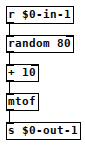
\includegraphics[scale=0.5]{images/pd-1.png}
        \caption{$f_1, f'_1$: note generator.}
    \end{subfigure}
    \begin{subfigure}{0.21\textwidth}\centering
        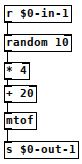
\includegraphics[scale=0.5]{images/pd-2.png}
        \caption{$f_2$: note generator, at a lower tempo.}
    \end{subfigure}
    
    \begin{subfigure}{0.21\textwidth}\centering
        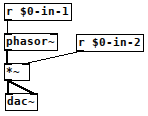
\includegraphics[scale=0.5]{images/pd-3.png}
        \caption{$f_3$: synthesizes the input note, sets the volume.}
    \end{subfigure}
    
    \begin{subfigure}{0.21\textwidth}\centering
        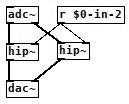
\includegraphics[scale=0.5]{images/pd-4.png}
        \caption{$f_4$: high-pass filter.}
    \end{subfigure}
    \begin{subfigure}{0.21\textwidth}\centering
        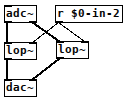
\includegraphics[scale=0.5]{images/pd-5.png}
        \caption{$f_5, f'_5$: low-pass filter.}
    \end{subfigure}
    \caption{The functions we use in our example, as defined in Pure Data.}
    \label{fig.pdpatches}
\end{figure}

\subsection{Reference implementation}
An implementation is being developed as an extension to the OSSIA library\footnote{\url{https://github.com/OSSIA/libossia}} and i-score software\footnote{\url{http://www.i-score.org}}. 
This implementation uses PureData~\cite{puckette1996pure} through libpd~\cite{brinkmann2011embedding} to provide function execution with multiple ports with primitives useful for musical creation. 
As such, it allows to work with audio, midi, and messages.

The C++ implementation of the execution algorithm, provided in the OSSIA library, is not tied in any way to PureData or any other environment: PureData is used as an example of implementation of a node to leverage an easy and well-known method to produce generators and filters with different kinds of inputs and outputs, which allows to cover the whole set of features.
Other nodes can be implemented through inheritance of a set of C++ classes.
As such, the processes currently available in i-score (automations, Javascript code, MIDI piano roll) and in i-score-audio (sound file reading, Faust and LV2 effects) are being ported to this new execution model.

In terms of user interface, PureData patches appear as nodes with their inputs and outputs in i-score.
There are two views: the main view, temporal and hierarchical, which allows to position the nodes in time, draw automations, etc., and the patching view which allows to connect nodes together and set the relationship types.
The temporal view instead has easily accessible text fields that allow setting input and output addresses for each port.

\section{Applied example: generative music}
\begin{figure}
    \centering
    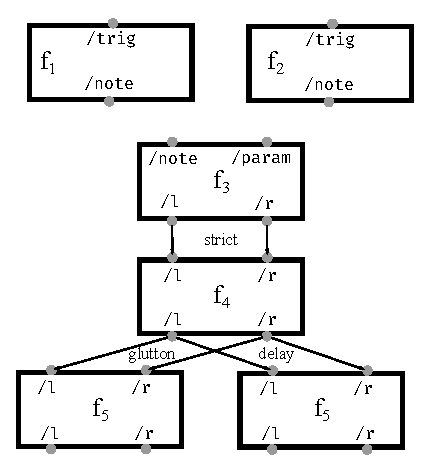
\includegraphics[scale=0.7]{images/nodes.eps}
    
    \caption{The dataflow relationships between instances of $f_{1,..5}$ in the program. The global environment contains variables for \lstinline|/vol| and \lstinline|/filt| when the execution starts. A PureData patch with similar semantics would use additionally \lstinline|throw~, catch~, send, receive, delwrite~, delread~,tabwrite~, tabread~| between nodes, and UDP \& OSC receivers and senders to read and write from the environment.}
    \label{fig.datapatch}
\end{figure}~
\begin{figure}
    \centering
    \begin{tikzpicture}
    \fill (0, 26.7529) circle (0.075) ; % State.0 
\fill (0, 27.9828) circle (0.075) ; % State.1 
\fill (0.510397, 27.9828) circle (0.075) ; % State.2 
\fill (1.30435, 27.9828) circle (0.075) ; % State.3 
\fill (2.00378, 27.9828) circle (0.075) ; % State.4 
\fill (2.68431, 27.9828) circle (0.075) ; % State.5 
\fill (2.9017, 27.9828) circle (0.075) ; % State.6 
\fill (4.07372, 27.9828) circle (0.075) ; % State.7 
\fill (0.283554, 26.7529) circle (0.075) ; % State.8 
\fill (1.51229, 26.7529) circle (0.075) ; % State.9 
\fill (0, 25.3529) circle (0.075) ; % State.10 
\fill (1.20983, 25.3529) circle (0.075) ; % State.11 
\fill (3.10019, 25.3529) circle (0.075) ; % State.12 
\fill (1.20983, 24.1231) circle (0.075) ; % State.13 
\fill (2.0794, 24.1231) circle (0.075) ; % State.14 
\fill (2.0794, 23.9717) circle (0.075) ; % State.15 
\fill (3.75236, 23.9717) circle (0.075) ; % State.16 
\fill (4.06427, 23.9717) circle (0.075) ; % State.17 
\fill (5, 23.9717) circle (0.075) ; % State.18 
\draw[line width=1pt] (0, 27.9828)  -- (0, 25.3529) ; % TimeNode.0 
\draw[line width=1pt] (0.510397, 27.9828)  -- (0.510397, 27.9828) ; % beau14cape47 
\draw[line width=1pt] (1.30435, 27.9828)  -- (1.30435, 27.9828) ; % free34jury66 
\draw[line width=1pt] (2.00378, 27.9828)  -- (2.00378, 27.9828) ; % cape36arch45 
\draw[line width=1pt] (2.68431, 27.9828)  -- (2.68431, 27.9828) ; % lola38oslo83 
\draw[line width=1pt] (2.9017, 27.9828)  -- (2.9017, 27.9828) ; % chat16band97 
\draw[line width=1pt] (4.07372, 27.9828)  -- (4.07372, 27.9828) ; % crop78zinc70 
\draw[line width=1pt] (0.283554, 26.7529)  -- (0.283554, 26.7529) ; % pews15apes27 
\draw[line width=1pt] (1.51229, 26.7529)  -- (1.51229, 26.7529) ; % cool83suds46 
\draw[line width=1pt] (1.20983, 25.3529)  -- (1.20983, 24.1231) ; % torr14siva73 
\draw[line width=1pt] (3.10019, 25.3529)  -- (3.10019, 25.3529) ; % bail5fred35 
\draw[line width=1pt] (2.0794, 24.1231)  -- (2.0794, 23.9717) ; % glom8deck49 
\draw[line width=1pt] (3.75236, 23.9717)  -- (3.75236, 23.9717) ; % rosa78holm28 
\draw[line width=1pt] (4.06427, 23.9717)  -- (4.06427, 23.9717) ; % bask79swat94 
\draw[line width=1pt] (5, 23.9717)  -- (5, 23.9717) ; % swig5mats22 
\draw[line width=1pt] (0, 27.9828)  -- (0.510397, 27.9828) ; % etch89star46 
\draw[line width=1pt] (0.510397, 27.9828)  -- (1.30435, 27.9828) ; % f1 
\draw[line width=1pt] (0.510397, 27.8828)  rectangle  (1.30435, 26.8828) node[pos=0.5] {$f_1$} ;
\draw[line width=1pt] (1.30435, 27.9828)  -- (2.00378, 27.9828) ; % daze85told77 
\draw[line width=1pt] (2.00378, 27.9828)  -- (2.68431, 27.9828) ; % f2 
\draw[line width=1pt] (2.00378, 27.8828) rectangle  (2.68431, 26.8828) node[pos=0.5] {$f_2$}  ;
\draw[line width=1pt] (2.68431, 27.9828)  -- (2.9017, 27.9828) ; % sept13hail24 
\draw[line width=1pt] (2.9017, 27.9828)  -- (4.07372, 27.9828) ; % f1.1 
\draw[line width=1pt] (2.9017, 27.8828) rectangle  (4.07372, 26.8828) node[pos=0.5] {$f_1$}  ;
\draw[line width=1pt] (0, 26.7529)  -- (0.283554, 26.7529) ; % shod51kola11 
\draw[dashed,line width=1pt] (0.283554, 26.7529)  -- (1.51229, 26.7529) ; % f3 
\draw[line width=1pt] (0.283554, 26.6529) rectangle (1.51229, 25.6529)  node[pos=0.5] {$f_3$}  ;
\draw[line width=1pt] (0, 25.3529)  -- (1.20983, 25.3529) ; % hail2dirt86 
\draw[line width=1pt] (1.20983, 25.3529)  -- (3.10019, 25.3529) ; % f4 
\draw[line width=1pt] (1.20983, 25.2529) rectangle (3.10019, 24.2529) node[pos=0.5] {$f_4$}  ;
\draw[line width=1pt] (1.20983, 24.1231)  -- (2.0794, 24.1231) ; % ramp43slug81 
\draw[line width=1pt] (2.0794, 23.9717)  -- (3.75236, 23.9717) ; % f5 
\draw[line width=1pt] (2.0794, 23.8717) rectangle (3.75236, 22.8717)  node[pos=0.5] {$f_5$} ;
\draw[line width=1pt] (3.75236, 23.9717)  -- (4.06427, 23.9717) ; % pies69year76 
\draw[line width=1pt] (4.06427, 23.9717)  -- (5, 23.9717) ; % f5.1 
\draw[line width=1pt] (4.06427, 23.8717) rectangle (5, 22.8717)  node[pos=0.5] {$f_5$} ;

    \end{tikzpicture}
    \caption{The temporal relationships between instances of $f_{1,..5}$ in the program.}
    \label{fig.timepatch}
\end{figure}

We present here an example that leverages patches built with Pure Data\cite{puckette1996pure}.
Figure~\ref{fig.pdpatches} present the Pd patches used. Fig.~\ref{fig.datapatch} presents the data relationships between the Pd patches, with the mapping of inputs and outputs to addresses of the environment. 
The inlets and outlets are ordered so that audio ports come first and message ports come afterwards.
Finally, fig.~\ref{fig.timepatch} presents the temporal score that orchestrates the execution of the Pd patches.

The execution happens as follows: 
\begin{enumerate}
    \item For a few milliseconds, nothing happens.
    \item $f_3$ is started. However, there is a strict dependency between $f_3$ and $f_4$: no sound is produced; $f_3$ is disabled.
    \item $f_1$ is started. Since $f_3$ is disabled, it writes \lstinline|/note| to the environment.
    \item $f_1$ stops, and a few milliseconds afterwards, $f_4$ starts, which allows  $f_3$ to execute. $f_3$ uses the last value of \lstinline|/note| that was put in the global scope by $f_1$.
    $f_3$ fetches the value of \lstinline|/vol| in the environment and $f_4$ fetches the value of \lstinline|/filt| there as well.
    Notice that $f_3$'s parent time constraint is dashed: it will execute until it is manually stopped.
    
    The sound that can be heard is a single tone with some amount of high-pass filtering.
    \item $f_2$ starts: random notes will be generated at a lower tempo and put at the \lstinline|/note| input of $f_3$ directly, bypassing the environment.
    
    \item $f_5$ starts: the low-pass filter adds itself after the high-pass filter.
    \item $f_2$ stops: the sound reverts to a continuous tone (the last that was written, again).
    \item $f'_1$ starts: tones are generated again, but with a faster tempo.
    \item $f_4$ stops: there is no sound anymore due to the strict dependency. $f_5$ applies its low-pass filter to silence.
    \item $f_5$ stops, and just afterwards $f'5$ starts. Since $f'5$ was in a delayed relationship with $f_4$, the sound produced corresponds to the sound that was heard at the beginning of $f_4$, with both $f_4$'s high pass filtering, and $f'5$'s low-pass filtering.
\end{enumerate}
\section{Conclusion}
Throughout this paper, the effects of adding macro-temporal semantics to dataflows were studied. 
The first step is to introduce an environment that allows execution of a program to continue if not all the nodes of a dataflow are currently being executed.
Then, we study the new possibilities offered by the presence of the environment by the different ways to interpret the absence of execution of a node.
This includes matching nodes together through pattern matching, and distinct policies of execution that can take into account the evolution of the program in time.

Such global environments have been implicitly present in multiple dataflow-based software; however they are not given an explicit existence. For instance, Max externals generally handle their global state through \lstinline|static| C variables. Making it explicit allows for better understanding of the execution of a program, and may enable further optimization opportunities.

After discussing the various choices left to the implementor, an example leveraging multiple PureData patches scheduled through an i-score score is explained.

A further goal for this work is to extend the definition not only to work with a single variable of time, but to any kind of activation mechanism: for instance, evolution of a position in a 3D space, etc.

The paper mostly centered around a single dataflow. A meaning has been proposed for multiple dataflows: they could be used as distinct variable scopes. If the temporal graph has hierarchical features, its use as a scoping mechanism should also be envisioned.
% TODO video / shader
\printbibliography

%Additional consideration: see PLOP 2006 article (multi-stream, etc), sample accuracy, etc
    
%Generalization to not only a single variable of time, but any kind of driving parameters


\end{document}
